\documentclass[12pt,twoside,vi]{mitthesis}
\usepackage[T1]{fontenc} % font encoding
\usepackage[numbers]{natbib}
\usepackage{graphicx}
\PassOptionsToPackage{hyphens}{url}\usepackage{hyperref}
\usepackage{color}
\newcommand{\draft}[1]{{\color{blue} #1}}
\newcommand{\wip}[1]{{\color{red} To do...}}
% \newcommand{\wip}[1]{{\color{red} #1}}
\begin{document}
\title{Git-Based Platform for Distributed Learning Communities}
\author{Vahid Fazel-Rezai}
\department{Department of Electrical Engineering and Computer Science}
\degree{Master of Engineering in Computer Science and Engineering}
\degreemonth{June}
\degreeyear{2018}
\thesisdate{May 25, 2018}
\supervisor{Philipp Schmidt}{Research Scientist, Director of Media Lab Learning Initiative}
\chairman{Katrina LaCurts}{Chairman, Department Committee on Graduate Theses}
\maketitle
\cleardoublepage
\setcounter{savepage}{\thepage}
\begin{abstractpage}
Instructors use software called learning management systems to administer online courses. Traditionally these digital platforms mimic physical classrooms, but new technology opens up potential for interactions not previously possible. In this thesis, we build a learning management system on top of Git to create a learning environment that encourages collaboration and exploration. We discuss how it was designed following established learning principles, the technical implementation, and the results of a pilot online class, with 100 learners lasting 6 weeks, as part of the Refugee Learning Accelerator. The platform architecture used in this study can be replicated and reused for other online courses with similar goals.
\end{abstractpage}
\cleardoublepage
\section*{Acknowledgments}
\wip{Acknowledgments...}

\tableofcontents

\newpage
\listoffigures

% \newpage
% \listoftables

\chapter{Introduction}

New education technology, enabled by the Internet, has allowed learners to connect with their instructors and with each other digitally. Pieces of software known as learning management systems take the experience of a classroom online, giving remote learners more access to education and enriching their learning experiences with a variety of technology.

In this thesis I employ Git, a version control technology initially created for collaboration among software developers, as the foundation for an experimental learning platform. The decentralized nature of Git can be utilized to expand interactions beyond replicating a traditional course. New interactions can be designed to balance the benefits of a collective learning experience with those of independent open-ended projects. In this study, I develop a prototype of such a platform, deploy it as part of an online course pilot, and examine the results. With this work, I hope to contribute to lowering the barrier of entry to administer an online course using a Git-based learning platform. The architecture I designed can be built upon in future courses. 

The following sections outline the research methodology of this study. Chapters 2 and 3 cover the theoretical background and other similar projects that were taken as guidance in designing the new platform. Chapter 4 steps through the design and implementation of the platform. Finally, results of a pilot run of using the platform in an online course are presented in chapter 5. 

\section{Refugee Learning Accelerator}

The development of a Git-based learning platform is part of a larger project called the Refugee Learning Accelerator (RLA). RLA is a program run by the Learning Initiative, a group of the MIT Media Lab. The goal of the program is to gather and support technologists from the Middle East to work on education tools for refugee learners. 

\draft{The program ran in three phases from fall of 2017 through spring of 2018. First, interested candidates applied as teams through an open process. Around 100 participants were selected for the first phase of the program, which consisted of a 6-week online course during November and December of 2018. The course operated on a weekly cycle:
\begin{itemize}
\item Challenge materials released every other week introducing a new technology. Teams were asked to design and build a prototype of a solution related to refugee education using that technology.
\item Twice during the week a webinar was conducted where an expert in the field discussed the week's technology and answered questions.
\item Teams were given independence to work as they liked over the course of the week.
\item Teams received qualitative feedback every week from the instructors once a week, at the midpoint and the end of each challenge.
\end{itemize}
The topics chosen for the online course were chatbots, human centered design, and AR. A description of each challenge is included in Appendix A.}

The second phase of the program brought 14 selected teams together for a week-long, in-person workshop in Amman, Jordan. There, teams forged their project ideas through rapid iterations of feedback and field observation. One important goal of the workshop was to foster a supportive community, where members encourage one another to pursue their projects and share resources.

Following the workshop, teams worked independently to bring their projects to fruition in partnership with local NGOs and with the continued support of the RLA community and Media Lab staff.~\cite{rla}

RLA is the product of the collective effort by members of the Learning Initiative and others passionate about finding creative ways to nurture learning, including the motivated participants, many of whom were working on their projects meanwhile also taking on a full-time load at work or as a student. The team of instructors included researchers and students from MIT and other affiliated experts. Mentors and speakers from all backgrounds donated their time to assisting teams through the webinars and at the workshop. The development of a learning platform a key one component in the operation of creating and executing the RLA program. 

While one of my goals in building the platform was certainly to support the online course of RLA, I also hoped to explore the possibilities of a Git-based platform. In this way, the online course of RLA served also as a pilot run for the platform in order to evaluate its utility and shortcomings. 

\section{Methodology}

Ultimately the research question I hope to answer in this thesis is: how can Git be used and adapted to support effective online learning communities?

This can be approached in three steps:
\begin{itemize}
\item First, I turn to established theory on digital learning pedagogy and principles to guide the characteristics and ultimately define interactions of the platform. In particular, I derive these interactions from first principles of learning and target learning outcomes rather than by attempting to move traditional classroom interactions online.
\item Second, I implement a technical platform that supports these interactions. The bulk of this work is done before the pilot course, but also includes the technical operation of the course. As much as possible, I rely on third-party software to increase reliability, reproducibility, and familiarity.
\item Third, I use the pilot run to evaluate not only how these interactions work in the manifested platform, but also how well they work. In order to gather feedback, I conduct an anonymous online survey among course participants. The survey questions are included in Appendix B. Responses to the survey as well as anecdotal evaluation are reported in Chapter 5.
\end{itemize}

The code and course content are all freely available online for use in future iterations of such research.~\cite{rla}

\chapter{Background}

Educational theory and pedagogy comprise a vast field and have been subjects of study since long before the advent of online education. Here we briefly touch on frameworks that went into consideration for this thesis. 

\section{Traditional Learning Platforms}

An online platform to support learning is not a new concept. A learning management system (LMS) is a tool that helps instructors supervise an online course, and popular commercial LMSs exist such as Blackboard, Moodle, and Canvas. 

A traditional LMS typically provides features including tracking learner grades, file management for assignments and corresponding submissions, and communication mechanisms for instructor announcements or learner questions. These features are often convenient duplicates of the same in-person interactions of traditional classrooms. Furthermore, as LMS is designed to complement traditional classrooms, it usually does not fully encompass the activities of a class, and an all-online course would require a medium of instruction external to the LMS.~\cite{zagalsky2015emergence}

Of note, the issue of learner collaboration, which is often a component of more creative, project-based assignments, is often not fully addressed in traditional LMS platforms. This intersection of collaboration and technology is instead known as computer-supported collaborative work (CSCW), and families of tools exist to support online collaboration. Learners thus would have to take to these external tools to collaborate, depending on the particular assignment.

\section{Foundational Theory}

\subsection{Self-determination Theory}

I begin with the assumption that humans have innate desire and ability to pursue their interests, and treat the role of the learning environment as fostering the right conditions. This is formalized in self-determination theory (SDT), which delineates three intrinsic pyschological needs:
\begin{itemize}
\item Autonomy: to see oneself as the causal agent of one's life.
\item Relatedness: to interact and connect with others in one's environemnt.
\item Competence: the accumulation of skills and ability to accomplish tasks.
\end{itemize}
SDT suggests that when these three feelings are present, humans are optimally disposed to grow.~\cite{ryan2000self}\cite{selfdetermination2}

The implication of SDT for design of a learning environment is to provide opportunities and encourage learners to be self-driven and motivated to explore their interests. Taking this perspective, not only can the learning environment cultivate ways of providing for the three basic needs prescribed by SDT, but can also channel learners' assumed individual motivation into achieving the desired learning outcomes.~\cite{selfdetermination}\cite{niemiec2009autonomy}

\subsection{Learning Outcomes}

We chose learning outcomes that align with the larger purpose of the RLA program and with consideration of the backgrounds of instructors and participants. 

On a broad level, we borrow objectives of learning from what is commonly used at the Media Lab and in particular often referenced by Mitch Resnick of the Lifelong Kindergarten group: design creatively, reason systematically, and work collaboratively.
These are not specific to RLA, but we can refer back to these general principles when defining specific deliverables. In particular, we can frame specific objectives in terms of the abilities of learners to think, learn, and work, as opposed to reaching a pre-defined state.~\cite{roleofmaking}

In the case of RLA, we are aiming for participants to continue beyond the course in building technologies for refugee learners, which involves outcomes in all three categories:
\begin{itemize}
\item Think creatively about new ways of utilizing technology for learning in unconventional settings.
\item Learn systematically how to find and employ the latest technologies.
\item Work collaboratively with other technologists, NGOs, and instructors to put a solution into practice.
\end{itemize}
The spirit of these outcomes can be found in the choice of challenge topics and deliverables (see Appendix A).

\subsection{The 4 P's}

We've established through SDT that learners can be self-driven, and that we would like to somehow cultivate a learning environment that channels this towards certain broad outcomes. Here we fill that gap. We lay out a framework for fostering creative learning based on four core components, the four P's of creative learning~\cite{cultivating}\cite{resnick2014give}\cite{creativelearningfuturework}:
\begin{itemize}
\item \textbf{Projects.} Project-based courses forces learners to design creatively and provides space for learners to realize their own vision.
\item \textbf{Peers.} Learning as part of a community not only feeds the relevance component of SDT, but also sets up learners to work collaboratively and build upon each other's work.
\item \textbf{Passion.} From SDT we take that learners are motivated by the ability to pursue areas of their own interest. We build this into the learning experience by allowing learners to work on what they care about.
\item \textbf{Play.} In our learning outcomes, there is no preset finished product of learning. The same applies to the process. Allowing learners to tinker and experiment with ideas can help them find the best learning experience for themselves.
\end{itemize}
We center the design of the learning platform on these 4 P's going forward. 

\section{Design Tensions}

Traditional courses emphasize delivering content through lectures, assignments, readings, and evaluations. The 4 P's call for some of the same aspects of traditional courses, but also an aspect of community that must be reconsidered in an online setting. Pulling these together creates tension between ``course'' and ``community'' and requires reconciling opposing characteristics of the learning experience:
\begin{itemize}
\item \textbf{Individual pathways vs shared experiences.} Learners prosper when given independence to really focus on their passions, but would then potentially miss out on experiences on which community can be built. 
\item \textbf{Team work vs solitary work.} Working in a team adds a feeling of belonging, but takes away from the autonomy component of SDT.
\item \textbf{Content vs connection.} Some experiences are great for conveying information that is ultimately needed to learn systematically, but would take away from the unstructured time in which learners can form their own connections.
\end{itemize} 
For each of these tensions, there are clear benefits on both sides to learning. Ideally, a learning experiences mixes and balances both sides of each tension.\cite{learningcreativelearning} 

There are other tensions where our pedagogy stands clearly on one side of the debate:
\begin{itemize}
\item \textbf{Projects vs puzzles.} Projects are open-ended and allow learners to be creative and work along the best path for them. With puzzles, the path to a solution has been decided by the instructor and creativity is removed from the experience.
\item \textbf{Open vs closed.} Collaboration and self-driven discovery are much easier when course content and others' work is visible to everyone.
\item \textbf{Qualitative feedback vs objective rubric.} A rubric inherently assume that there is a set of checkboxes towards which learners work, again removing creativity and limiting exploration. On the other hand, constructive feedback not only tailors evaluation to the type of work that is best for the learner, but also can be used to encourage further play. Additionally, peer feedback connects learners with each other and enhances the community feeling.
\end{itemize}
We consider features of the platform and the facilitation of the RLA course along these dimensions.

\chapter{Related Work}

In this chapter we survey existing technologies and platforms that we can learn or borrow from in developing a Git-based learning platform. Git has been applied to many fields, and its application to education has recently come under study by researchers.

\section{Overview of Git}

Git is a technology that is used for online collaboration, particularly in software engineering. Created in 2005 by Linus Torvalds as a tool to support the development of the Linux kernel, Git allows users to each have a local copy of a set of files and sync between their copy and a central server in a coordinated fashion. Git is also a version control system, hence allowing users to backtrack changes or split into multiple branches of work from the same starting state.~\cite{githistory}

Git is used as a command line tool, in which users type text commands to perform the desired git actions, but there are also graphical interfaces available which serve as a wrapper and replacement for the command line. On top of Git, hosting services such as Github, GitLab, and Bitbucket provide a range of features that are as integral to some workflows as Git itself.~\cite{githosting}

Overall, the benefit of Git derives from its powerful capabilities as a collaboration tool, but comes with the cost of an upfront time investment to learn its operation.

\section{Communities of Practice}

A community of practice consists of a group of people, a common interest that they share, and interactions or activities where the group acts on their interest. Members of the community learn from each other and improve their practice. Software development is an example of a community of practice, and Git was created to address the issue of collaboration on code in such a community.~\cite{teachingdigital}

\draft{Git has gone on to prove useful in other communities of practice and has been adapted for collaboration in areas other than code.~\cite{sevenwaysgit} The community of an online course can itself be seen as a community of practice, so other applications of Git may bear lessons on how to adapt it for learning.}

\section{Other Uses of Git}

\draft{
While Git was initially created for and is actively used by the software development community, its application has spread to many other use cases:

\begin{itemize}
\item \textbf{Programming-based courses.} Initially used for collaborating on work, Git is making its way into classrooms as a form of submitting work as well. Instructors may even set up repositories for students for their use or collaboration with teammates.~\cite{whygithubclassroom} Github itself has even added features to streamline this use case.~\cite{githubclassroom} However, note that this is not a LMS and usually is not used as a complete learning platform.
\item \textbf{Contest submission.} DevArt by Google ran a contest for which they provided a template repository and submissions were accepted by taking advantage of Github's fork functionality. The template repository was forked over 2000 times.~\cite{devart} Similarly, Mozilla accumulated submissions for its Global Sprint event using the issues feature on Github.~\cite{globalsprint}
\item \textbf{Project management.} Communities of practice centered around a Git repository complete the workflow by using issue tracking (built into Github) and real-time chat services in conjuction with the codebase.~\cite{githubpm}
\item \textbf{Datasets and legislation.} Git hosting platforms have the level of availability and navigation that make them suitable for hosting various collections of information including datasets and pieces of legislation.~\cite{sevenwaysgit}
\item \textbf{Blogging.} The version control aspect of git is often used as a content management system. Github provides support for serving files in Markdown format as static websites, which makes this even simpler.~\cite{whygithubclassroom}
\item \textbf{Recipes.} A service called Fork the Cookbook allows users can fork, or copy, an existing recipe and tweak it to make it their own. This creates a collaborative and decentralized platform for sharing cooking recipes.~\cite{forkthecookbook}
\item \textbf{Travel logging.} A Github user has a repository for his personal travels, where onlookers can submit suggestions for attractions in a city he is planning to attend by suggesting edits for that particular city's file.~\cite{travellog}
\end{itemize}

Synthesizing these applications, we summarize several key techniques in the adaptation of Git to power communities of practice:
\begin{itemize}
\item Using Git hosting platforms as a link-able and easily navigable host of information.
\item Using of version control and Markdown as a content management system.
\item Parsing files managed by Git as a static web page, as done by Github Pages.
\item Empowering members to contribute to a central file by submitting a suggested edit.
\item Creating a submission of work by forking a template repository and adding work to the forked repository.
\item Using group chats such to complement Git projects with more real-time communication.
\end{itemize}
}

\section{Suitability of Git for Learning Platforms}

\draft{While Git was not originally designed as a learning platform, we found in it suitable qualities. Here we discuss the benefits of git as a tool for fostering positive educational interactions.

First of all, Git aligns with the design tensions discussed above: 
\begin{itemize}
\item \textbf{Individual pathways vs shared experiences.} Git gives individuals the freedom to take a self-defined path of work by being flexible in how it merges back into the main body of work. Learners can use their preferred tools and platforms, since any file type is supported. At the same time, the project repository acts as a shared space that learners share and can interact with each other in.
\item \textbf{Team work vs solitary work.} Using Git allows learners to work independently on their own time, yet at the same time collaborate with teammates by building on each other's work. After all, its raison detre is to be able to build upon each others' work without conflict.
\item \textbf{Content vs connection.} Git can serve as a means of delivering educational content. As discussed in the previous section, Git can also be adapted as the underlying mechanism of a content management system. As a versioning system, Git enables publishing new content, updates, and revisions in a fashion that can be distributed. Popular git hosting websites such as Github and GitLab have built-in support for Markdown-formatted files and support and static web pages. At the same time, learners, can form connections with each other by reviewing each other's commits or suggesting edits to someone else's work. 
\end{itemize}

Git also aligns well with the preferences for the type of experience RLA is designed to be:
\begin{itemize}
\item \textbf{Projects vs puzzles.} Git gives learners room to play, since branches can be made to explore new ideas and unsuccessful changes can be easily reverted.  
\item \textbf{Open vs closed.} By default, everyone's is work openly documented and visible. Commit messages log a complete history of changes.
\item \textbf{Qualitative feedback vs objective rubric.} As a version control system, the currency is in units of iterative work rather than a final deliverable, reinforcing the idea that there is no preset rubric for what is considered good or bad work.
\end{itemize}

Finally, because Git is already widely-used, it is reliable in a techincal sense and help material is readily available online for easing adoption. On the flip side, Git's wise use makes it an important skill. Code collaboration is practically a requirement in the software development industry in particular, and software is increasingly relevant in all industries, so learning Git as part of a participating in course can itself be an additional benefit.~\cite{haaranen2015teaching}}

\chapter{Platform Development}

In this chapter we walk through the design and implementation of the Git-based platform. 

\section{Design}

In this section I lay out the high-level design for the RLA course. The platform and pedagogy are closely linked, but one does not necessarily imply the other. In other words, while a platform can be built to support a desired pedagogy, the content and facilitation are also critical to achieving it. On the other hand, a particular pedagogical approach may not be possible without a platform that can support it. 

Hence, the design must encompass the whole course, from which the platform design will follow. Though the design targets the goals of the RLA program, it is intended to be adaptable for other future courses.

\subsection{Balancing Tensions}

We consider the tensions outlined in Chapter 2 in a few key areas:
\wip{restructure subsection in terms of tensions instead of new areas}
\begin{itemize}
\item Teamwork. We allowed learners to apply as teams so that they self-select into groups. This allows learners to work in teams, but still feel autonomy over who their team is and how they work within their teams.
\item Communication. Communication lays the groundwork for the type of community formed. We aim to have instructors clearly communicate how to use the platform and be able to guide students throughout the course. General course information should be readily accessible to students. While this address content, we also want to address connectino. We allow for natural and structured opportunities to ask questions and give feedback. One of the secondary goals of the online coures is to foster a community that extends into the later phases of the Accelerator.
\item Permissions. We must decide how to control authority to perform actions and visibility of content. On one hand, we believe that the platform should be as open as possible. This would allow students the opportunity to pursue their curiosities, to learn from each other's work, and to feel that they have a complete understanding of the platform. On the other hand, we would like to prevent either intentional or accidental actions that may destroy or hinder other participants' work. We also anticipate that sensitive topics would not be expressed without a private way of doing so and thus would like to allow for that.
\end{itemize}

\subsection{Platform Interactions}

The details of the design were chosen to support the needs of RLA's weekly cycle. In each week of the cycle, content is released at the beginning and learners worked towards a particular milestone by the end of the week. Throughout the week learners can collaborate and participate in seminars.

To achieve these requirements, there are four interactions that the core Git-based platform needs to support:
\begin{itemize}
\item \textbf{Onboarding.} We want learners to be able to register for the course as easily as possible, yet still provide basic information to introduce themselves to the rest of the learner community. 
\item \textbf{Content distribution.} New material posted at the beginning of the week includes a description of the week's challenge and targeted milestones. In addition, resources relevant for the week are gathered and provided for learners' reference. This content may also sometimes include skeleton code or template documents in which learners can report their progress. These pieces of content require the additional ability of being pulled into learners' working directories.
\item \textbf{Collaboration.} Throughout the week, teams work together on a single project or codebase in some sort of team work space. 
\item \textbf{Submission.} At the end of the week, learners need a mechanism to put together a package representing the state of their work on which to receive feedback. We also encourage learners to use these submissions as a resource to learn from other learners' approach to the challenge.
\item \textbf{Feedback.} We believe frequent personalized feedback can be helpful to learners and also cultivates a culture of collaboration. Hence we'd like our platform to provide an interface where a reviewer can easily peruse a learner's work and leave comments. 
\end{itemize}
Note that all these interactions have similarity in structure with feature development and code review used in software engineering, so we can utilize corresponding features in the Git hosting service.

In addition to managing the course content, we also want to support a few additional types of communication:
\begin{itemize}
\item For seminars, we needed a way to broadcast video to learners. Additionally, we would like to engage learners to drive the conversation according to their passions and have face-time with their peers.
\item For technical support and other miscellaneous discussion, we would like to have an open, real-time, group chat. In particular, the group aspect will expose the entire community to conversations as appropriate so that everyone feels included and in-the-know.
\item For showcasing teams' work, especially to parties outside the course, it would be ideal to have a static website summarizing the challenges and the progress coming out of the course. Anyone could then share the link and in this way feel ownership over their work.
\end{itemize}

\section{Components}

\subsection{Git hosting service}

In order to have a group of distributed learners participate in the course using Git, we needed to have an server accessible by the Internet running Git where the content would be hosted. We looked at two of the most popular Git hosting services, Github and GitLab. Both offer a SaaS model where they host Git on their servers and simply provide an interface, as well as a self-hosted version where they provide the software but leave running a server to the customer.

We compared options the two in terms of features, styles, and technical performance.

The two options had very similar sets of features. Github has organizations, teams, repositories, and pull requests, while GitLab has groups, subgroups, projects, and merge requests. Both expose a webhook for Git commits, allow in-browser editing of files, and can serve hosted files as static websites. Both offer free or discounted private repositories/projects for educational uses. On a few points GitLab had additional features, such as being able to request to join a group and being able to trigger scripts that run before serving static websites.

Many software companies use Github to host either all their code or even just their open source projects, and as a result a Github profile feels very much like a professional portfolio. We wanted to make sure learners are comfortable experimenting and making mistakes, and took into consideration that some may feel less inclined to do so if the work would permanently be associated with their professional portfolio. 

Finally, we took into consideration the technical reliability of each option. We found that GitLab's SaaS offering, GitLab.com, was often slow to load. For both, a self-hosted instance would include considerable setup and costs to run a server, but would allow customizations such as the domain name. Finally, though both are welcoming homes to open source projects, Gitlab has made the web platform itself open source, whereas Github's is not.

For our course, we ended up opting for GitLab, and chose to mitigate performance issues by using a self-hosted instance of the free tier. However, it would certainly be possible to adapt our approach for either GitLab or Github, in the both SaaS and self-hosted models.

\subsection{Chat service}

To allow the development of a community, we wanted to make communication among learners as well as between learners and instructors as open as possible. GitLab alone, with commit messages and comments on merge requests, did not offer as fluid of a setting as we wanted. We decided to augment GitLab with a team-based chat service where learners could communicate in real time.

We looked at existing cloud messaging services including Slack, Gitter, and Mattermost, all of which have a very similar design. They provide open channels where any user can join and chat, as well as messaging between users and in private groups for more direct communication. We hoped to use these spaces as a forum for discussing ideas, asking each other for help, and even just to meet other learners.

From our options we chose to run a self-hosted instance of Mattermost, largely due to our choice of self-hosted GitLab. Mattermost and GitLab have a built-in integration for authentication and backend configuration. Mattermost is also open source, continuing in our spirit of relying on open source tools.

\subsection{Server infrastructure}

\draft{reliance on other software (letsencrypt, nginx, python and javascript, bash)}

\section{Technical Implementation}

In this section we outline the initial implementation of the platform. We assume a technical background, in particular familiarity with Internet architecture and Git.

\subsection{Server configuration}

\draft{The chosen components were open source pieces of software that required a server on which to install and run instances of these programs. Therefore the first step was to spin up and configure a network connected server. for this task I chose to use digitalocean but other service providers would have been equally valid choices. the server was configured as a Linux machine and could be accessed via SSH from any client. Next I downloaded and installed the gitlab Community Edition on the platform server. this version of get lab included and easy to use configuration file where all the settings of gitlab could be specified to the needs of the rla course. in this configuration the following settings were made. include itemized list of settings made forget lab here. to access get lab from the internet requires connecting a domain to the platform server and considering the platform server to Route request to this domain to be served by the running instance of get lab. on the external side this was accomplished by purchasing a domain for the rla course and then creating records in the domain name server to point that domain to the platform servers IP. on the server side, this routing was accomplished using nginx a default configuration of which was included in the get lab installation. however this default did not include secure SSL connection and therefore could not support https. to enable to port for https I created a certificate using the let's encrypt service for free. I then configured the nginx using custom configuration 2 use this certificate to authenticate secure connections and enable https for the gitlab website. at this point a usable gitlab instance was running on the platform server.

the next component of the platform was the mattermost group chat service. As with gitlab mattermost was provided in an easy to download and install open source software package. even more conveniently gitlab and it's configuration file allows for integration with mattermost already built in. in particular one of the key pieces of this integration was Authentication. Pi configuring the appropriate settings a user when now be able to register for the get Lab website and then use those credentials to login to the matter most portion of the website. As a result users would be consistent across these two platforms both facilitating the creation of the course community and also simplifying the experience for individual learners. to access mattermost from the internet a similar process was undertaken. I knew something was created and nameservers were updated with records to point the subdomain 2 the platform server period on the server side nginx was modified yet again to serve requests at this sub domain using both HTTP and https. mattermost was also configured to suit the needs of the are Lake course and channels where set up in advance to guy discussion around challenges support and social interaction.

with these two main components in place much of the configuration could be done through the corresponding web interface. for example a group was created for the Arlie course and configured with the appropriate permissions for joining the group and for editing particular projects.

DigitalOcean droplet https://www.digitalocean.com/community/tutorials/how-to-install-and-configure-gitlab-on-ubuntu-16-04 
GitLab [built in for DO]
NameCheap domain and networking
nginx customization
Lets encrypt}

\subsection{Git architecture}

\draft{motivate this

\begin{itemize}
\item \textbf{Divided by folder.} All teams commit to one shared master branch, but in different folders. The benefit of this approach is its simplicity, but the downside is the lack of permissions enforcement to avoid one team interfering with another's work.
\item \textbf{Divided by branch.} All teams commit to different branches of a single class repository. This way teams can even rebase on master to gain access to new course materials. Though tricky, it is also possible to enforce appropriate permissions so teams can only push to their own branch. The downside is that it becomes messy for teams to create their own branches for development.
\item \textbf{Divided by repository.} All teams work in their own repositories, which are pulled together each as a subtree within a course repository. This allows for complete freedom for teams within their own repository with simple permission settings, but creates complexity in having each team's work in multiple locations, namely in two separate repositories. 
\end{itemize}
}

\subsection{Custom Scripts}

\draft{As much as possible, Git-related operations of the platform were automated to ease the burden on the instructors. 
\begin{itemize}
\item Onboarding membership request poller
\item Onboarding group creation
\item Health check with email notifications
\item Create subtrees
\item Create merge request
\item Perform merge
\item Analyze progress
\end{itemize}
}


\chapter{Results of RLA Pilot}

For six weeks in November and December of 2017, approximately 100 learners participated in an online course using the Git-based learning platform as the first phase of the RLA program. Following the course, an optional survey was conducted, the questions of which are included in the appendix. In this section we report the experience, results, and feedback we observed in the course and survey responses.

\section{User Experience}

\draft{Frame around tensions, for each broad set of interactions go over "what did it look like", "how did it work", and "how well did it work"}

\begin{figure}[H]
\centering
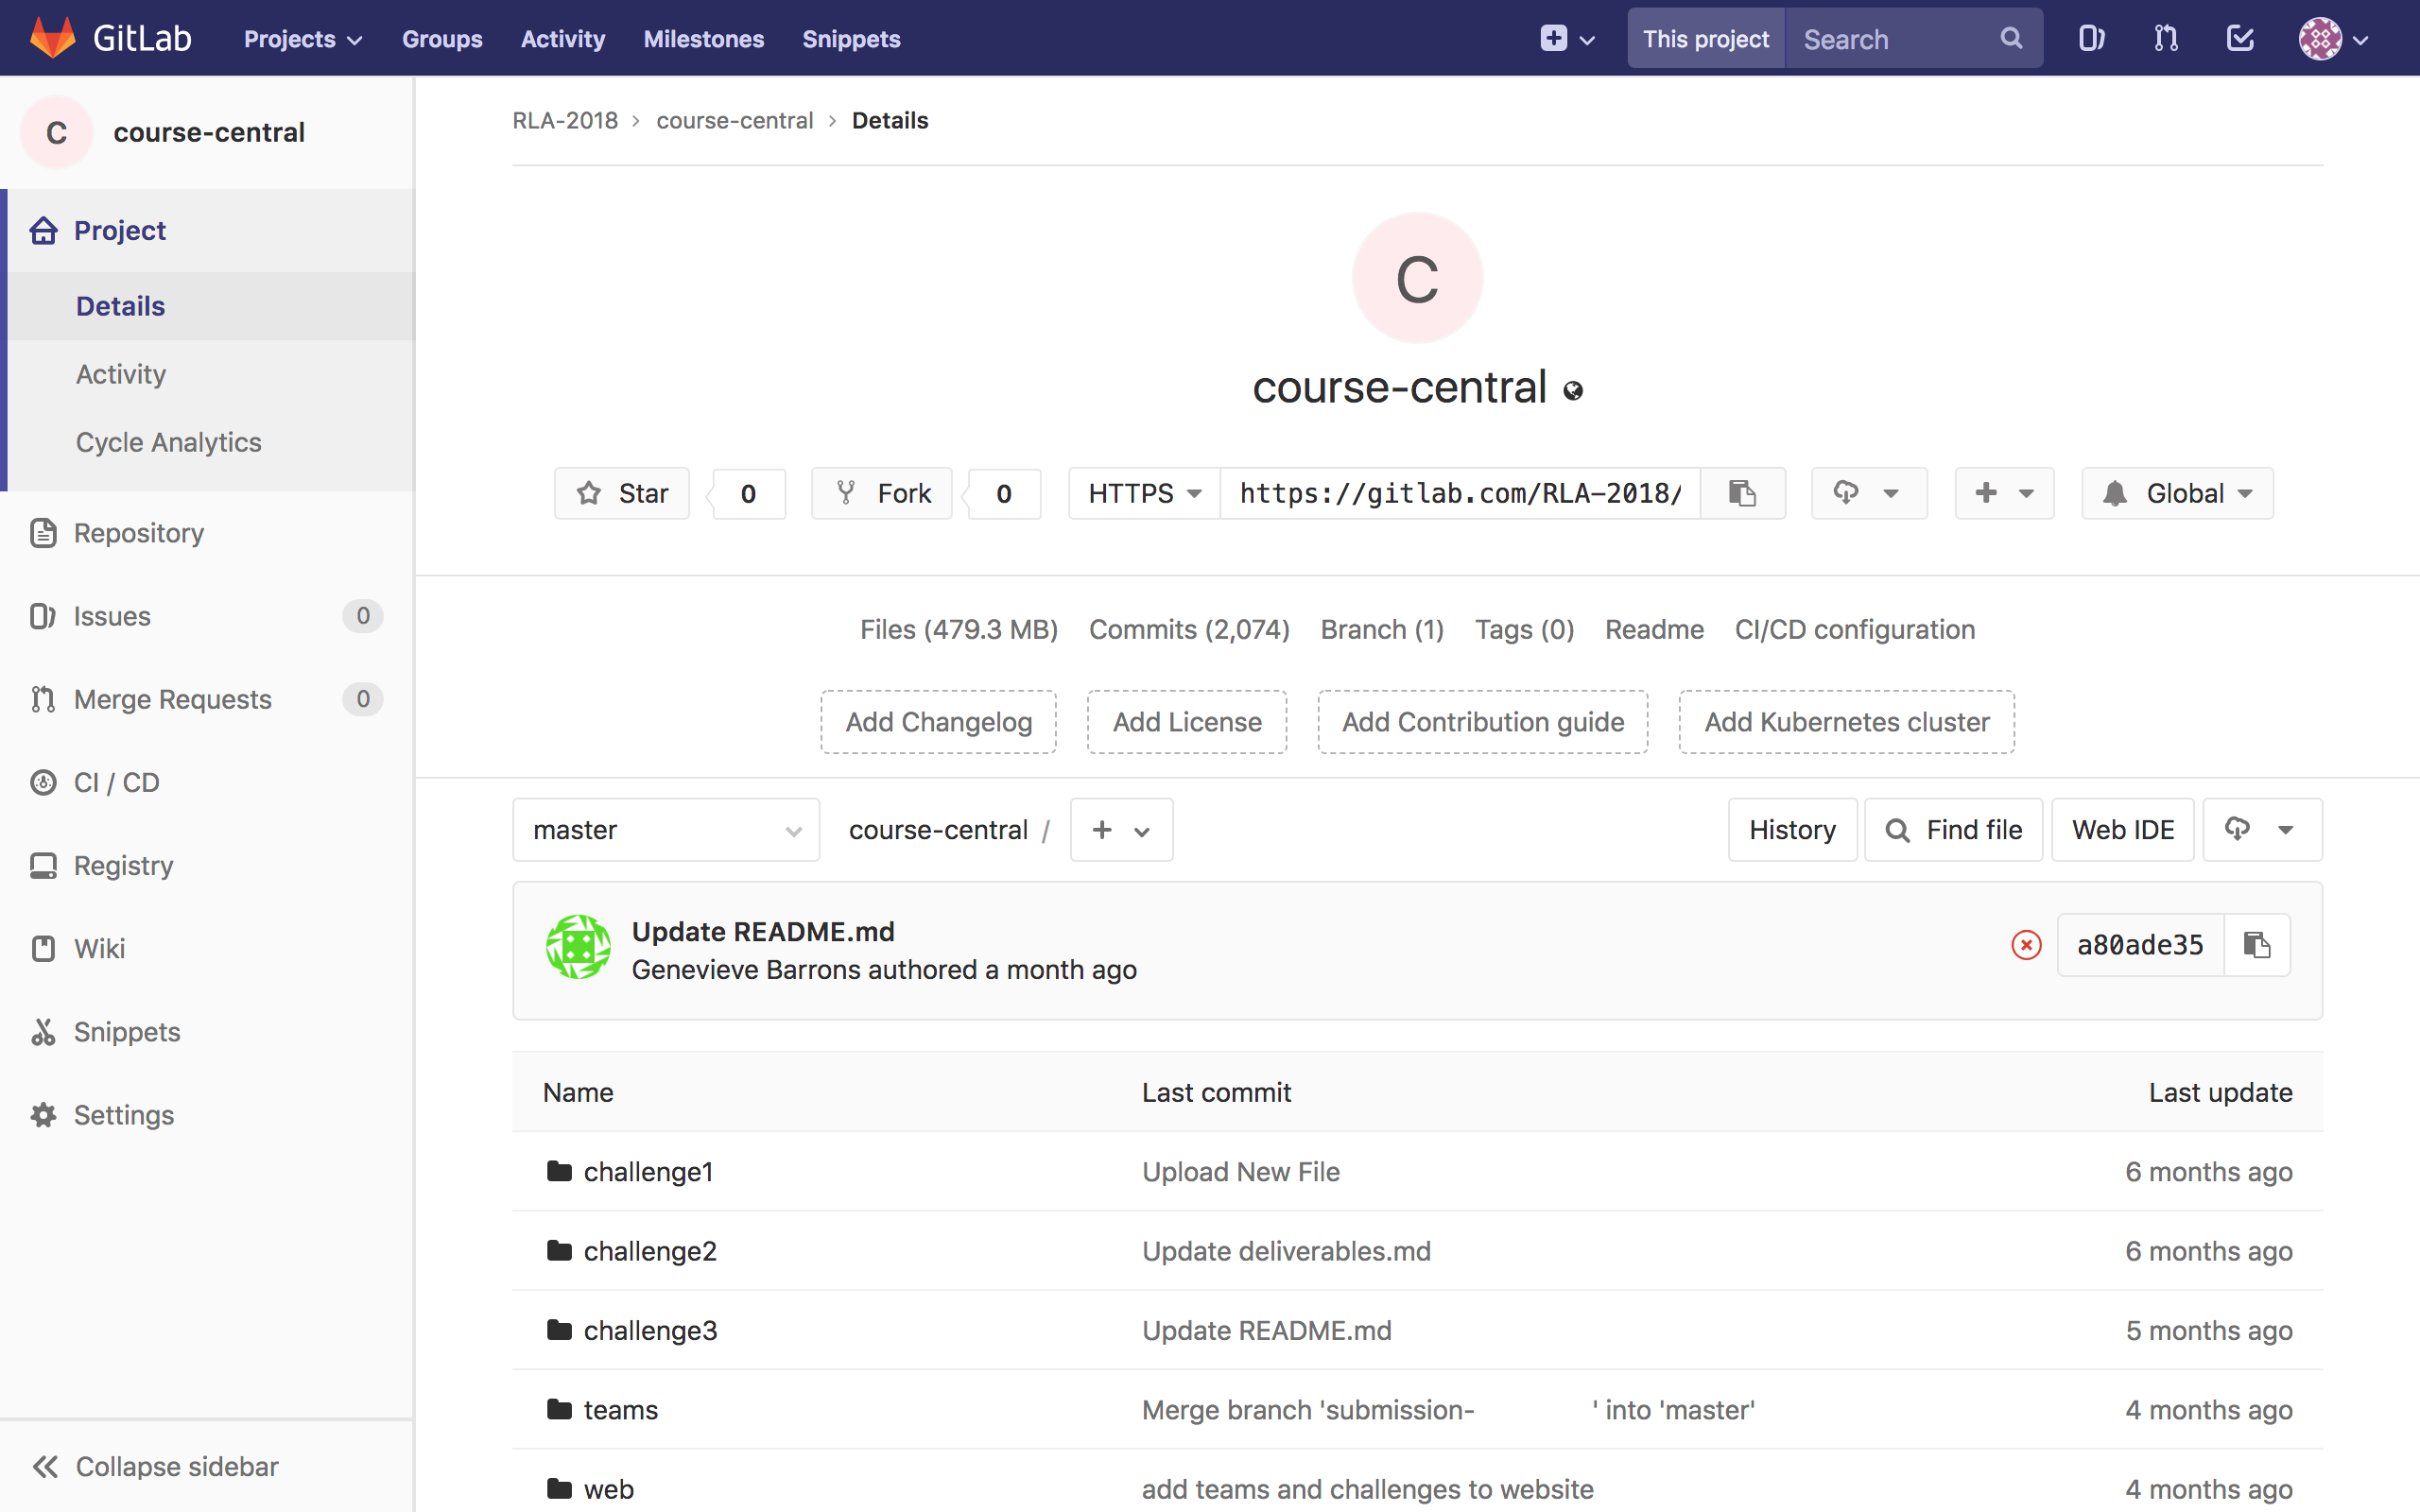
\includegraphics[scale=0.3]{fig-course-central.png}
\caption{The \texttt{course-central} repository.}
\end{figure}

\chapter{Conclusion}

\draft{narrative summary of thesis, an honest set of personal takeaways (from which reader can judge whether to replicate work) and feeligns about future work}

\appendix

\chapter{RLA Challenge Descriptions}

The online course was divided into three challenges, each of which had two sets of deliverables (one for each week). Here we provide brief descriptions of these. More information as well as various resources related to the topics of each challenge is available online.~\cite{rla} All content was developed by members of the MIT Media Lab Learning Initiative unless otherwise noted.

\begin{enumerate}
\item \textbf{Challenge 1 - chatbots:} How might we use chatbots to support refugee learners inside or outside of the classroom? 
\begin{itemize}
\item Describe your concept for a chatbot in one or two paragraphs. Use visuals (mockups, diagrams) if possible. It is important to be as specific as possible while mapping out the scope of the project as this will greatly influence implementation and the tools to use. Answer the following questions:
\begin{itemize}
\item What problem/ challenge will the chatbot solve? 
\item How will the chatbot solve it? 
\item Who is the primary user and how will the chatbot engage the user?
\item What activity does the chatbot facilitate that would not otherwise be possible? 
\item What challenges do you expect to encounter?
\end{itemize}
\item Demonstrate how your chatbot works. Videos, screenshots or images are encouraged. Add a short description and answer the following questions: 
\begin{itemize}
\item How did you build it? (Platform and technology)
\item What challenges did you face?
\item What aspect of the chatbot do you like best? 
\item What would you different in the future? 
\item Please also add a link to your code!
\end{itemize}
\end{itemize}
\item \textbf{Challenge 2 - human centered design:} How might we use everyday technologies as learning tools?
\begin{itemize}
\item Make an initial prototype. Questions to answer:
\begin{itemize}
\item What solution are you testing? (and why did you choose it?)
\item Submit your prototype (use photos, video, diagrams etc.)
\item Describe the prototype and why you chose this prototyping method. 
\item What did you learn during the prototyping process?
\item Who are your intended users for testing?
\end{itemize}
\item Test it with users. Questions to answer:
\begin{itemize}
\item How did you select your test users? 
\item What was the setting of the test? 
\item What were the main points of feedback you received (share a summary)? 
\item What changes would make to your idea/project based on the feedback?
\item What parts of the Human Centered Design process were new to you?
\item What parts of the Human Centered Design process seemed most useful to you?
\end{itemize}
\end{itemize}
\item \textbf{Challenge 3 - augmented reality (AR):} How might we use Augmented Realtiy (AR) to support refugee language learning outside the classroom?
\begin{itemize}
\item Describe your concept for how low fidelity Augmented Reality could be used to support language learning in one or two paragraphs. Use visuals (mockups, diagrams) if possible. It is important to be as specific as possible while mapping out the scope of the project as this will greatly influence implementation and the tools to use. Answer the following questions:
\begin{itemize}
\item What problem/challenge will the AR experience solve? 
\item How will the AR experience solve it? 
\item Who is the primary user and how will the AR experience engage the user?
\item What hardware does the user need? Is this realistic in the refugee context? 
\item What activity does the AR experience facilitate that would not otherwise be possible? 
\item What challenges do you expect to encounter? 
\end{itemize}
\item Demonstrate how your AR experience works. Videos, screenshots or images are encouraged. Add a short description and answer the following questions: 
\begin{itemize}
\item How did you build it? (Platform and technology)
\item What challenges did you face?
\item What aspect of the AR experience do you like best? 
\item What would you different in the future? 
\item Please also add a link to your code!
\end{itemize}
\end{itemize}
\end{enumerate}

\chapter{RLA Online Course Survey}

The following questions were sent in an email to participants to gather feedback and evaluate how well the platform worked. The survey was anonymous and asked for consent for responses to be used in this research study. A total of 11 participants chose to respond.

\begin{enumerate}
\item Git
\begin{itemize}
\item How much had you used Git before the course?
\item To what extent did you learn Git during the course?
\item How useful would you say knowledge of Git was for collaborating with your team?
\end{itemize}
\item Course materials
\begin{itemize}
\item Did you have any difficulty accessing course materials? If so, what were they?
\item Did you find the course materials helpful in working on your projects? If so, which materials were most helpful?
\end{itemize}
\item Signing up
\begin{itemize}
\item Did everyone on your team submit their own initial sign up on GitLab?
\item How many people on your team used GitLab after the initial sign up? Was there a reason some did not?
\item Did you find it useful to have a list of participants in the course?
\end{itemize}
\item Submission
\begin{itemize}
\item Would you have preferred an automatic, continuous submission (as opposed to your work being snapshot at a set time)?
\item Did you run into any issues in submitting your work? If so, what were they?
\item Were you able to see other team's submitted work? If so, did you find that useful?
\end{itemize}
\item Seminars
\begin{itemize}
\item What were your favorite and least favorite features of the Unhangout platform for seminars?
\item Did you find the seminars useful in ideating for your projects? If so, were any seminars particularly useful?
\item Did you find the seminars useful for the technical side of your projects? If so, were any particularly useful?
\end{itemize}
\item Team
\begin{itemize}
\item How was the technical work distributed among your team?
\item Was your team physically located in the same place?
\end{itemize}
\end{enumerate}

\clearpage
\newpage
\begin{singlespace}
\nocite{*}
\bibliography{sources} 
\bibliographystyle{apa}
\end{singlespace}
\end{document}


\wip{proofreed for tense and second person}